\bab{BAB I}{PENDAHULUAN}
\setcounter{chapter}{1}

\renewcommand{\thesection}{\thechapter.\arabic{section}}
\section{Latar Belakang}

Kendaraan otonom telah menjadi salah satu inovasi teknologi paling menjanjikan dalam sektor transportasi modern. 

\begin{figure}[H]
    \centering
    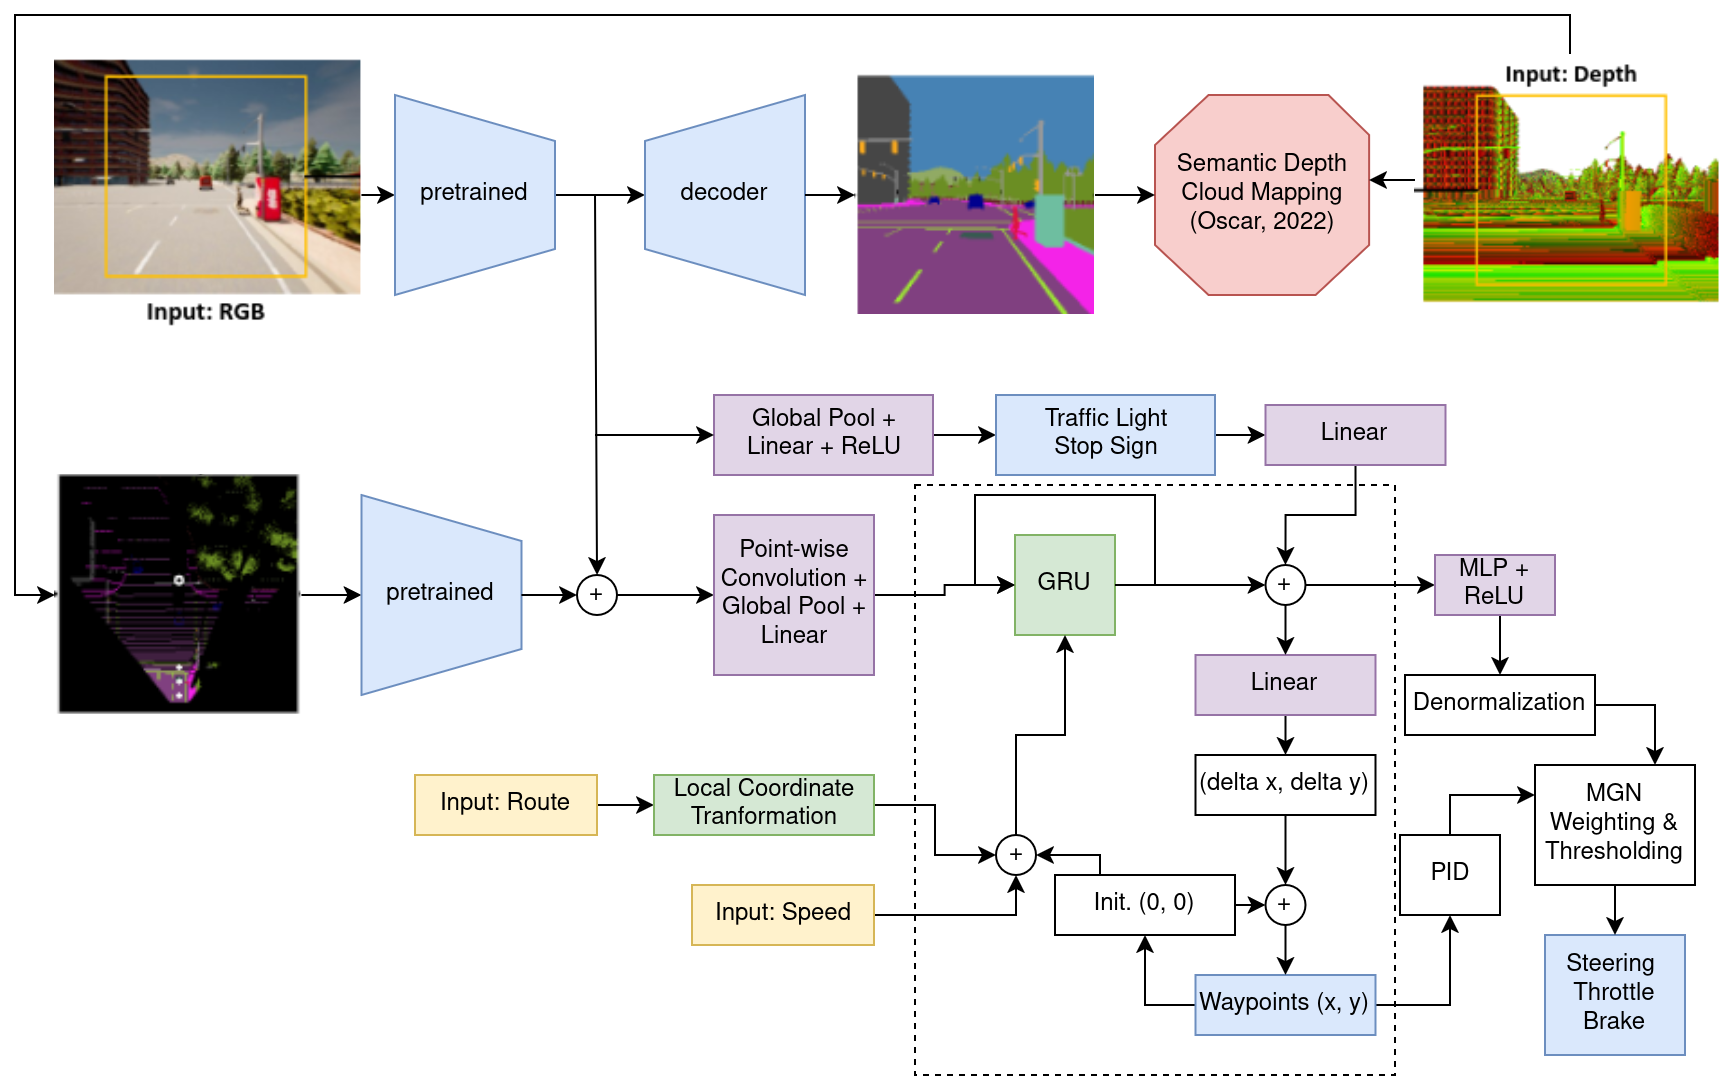
\includegraphics[width=1\textwidth]{images/architecture-x13.png}
    \caption{Arsitektur x13 \parencite{Natan2023-hi}.}
    \label{fig:architecture_x13}
\end{figure}

Pada Gambar \ref{fig:architecture_x13}, ditampilkan arsitektur x13 yang digunakan dalam sistem prediksi waypoints dan navigasi kendaraan otonom. Arsitektur ini terdiri dari beberapa komponen utama, termasuk EfficientNet sebagai backbone untuk ekstraksi fitur dari input RGB, Gated Recurrent Unit (GRU) untuk memproses data sekuensial dan menghasilkan prediksi waypoints, serta encoder untuk ekstraksi fitur dari semantic depth cloud. Dalam arsitektur ini, input berupa gambar RGB dan data kedalaman (depth) diproses melalui modul segmentasi untuk menghasilkan peta kedalaman semantic depth cloud (SDC), yang kemudian digunakan dalam proses pengambilan keputusan terkait navigasi.

\section{Rumusan Masalah}
\begin{enumerate}
    \item Bagaimana pemanfaatan arsitektur Transformer dalam komponen arsitektur berbasis CNN tradisional, seperti EfficientNet dan GRU, untuk meningkatkan performa prediksi waypoints dan navigasi pada kendaraan otonom?
    \item Apakah penggunaan Transformer mampu meningkatkan akurasi dan responsivitas sistem kendaraan otonom terhadap perubahan kondisi jalan yang dinamis?
    \item Apa saja kendala teknis yang muncul dalam penerapan arsitektur Transformer, khususnya terkait kebutuhan komputasi dan dataset pelatihan pada tugas multi-task learning untuk kendaraan otonom?
\end{enumerate}

\section{Batasan Masalah}
Dalam penelitian ini, terdapat beberapa batasan yang perlu diperhatikan untuk memperjelas ruang lingkup dan fokus studi yang akan dilakukan, antara lain:
\subsection{
    Lingkup Data Sensor yang Digunakan
}
Penelitian ini akan menggunakan data dari sensor kamera RGB-D dan informasi lokasi dari GPS untuk proses persepsi lingkungan dan pengambilan keputusan. Data dari sensor tambahan seperti LiDAR atau radar tidak akan dipertimbangkan dalam penelitian ini, sehingga hasil penelitian terbatas pada arsitektur yang mengandalkan data visual dan kedalaman dari kamera RGB-D.
